%plurals_event_chap_34
%PRECOMPILE COMMAND pdftex -ini -jobname="plurals_event_chap_34" "&pdflatex" mylatexformat.ltx plurals_event_chap_34.tex
\documentclass[english]{article}
\usepackage[T1]{fontenc}
\usepackage[latin1]{inputenc}
\usepackage[sort]{natbib}
\usepackage{stdprmbl}

\usepackage{parskip}

\lingset{interpartskip = -5pt}
\lingset{aboveexskip = 3pt,belowexskip = 3pt}

\definecolor{darkred}{rgb}{0.4,0,0}



\title{Plurals and events (chap. 4) : Essential Separation}
\author{Keny Chatain}

\begin{document}
\maketitle

\section*{Structure of the argument}

Schein attempts to show that the truth-condition of sentences like \cnextx{a} are unavailable if we assume that \quo{teach} denotes a 4-ary predicate (3 arguments of the verb + event)\footnote{Schein uses \emph{indirect} semantics, where a sentence first gets translated into a formula of some logical language, which itself receives a model-theoretic representation. I rephrase in terms of the more familiar \emph{direct} semantics of Heim and Kratzer, where sentences immediately translates to model-theoretic objects.}

\pex
\a Three video games taught every quarterback exactly two new plays. \label{quat}
\a \textbf{Observed truth-conditions:}\\
Every quarterback learned two new plays\\
They received instruction from three video-games.
\a \quo{teach} denotes an $eeevt$ predicate
\xe
%
An argument of impossibility is tricky to make: one needs to make sure that the reading is impossible to obtain under any auxiliary assumptions. In particular, Schein explores two classes of auxiliary assumptions:

\begin{enumerate}
\item \textbf{Composition:} how quantifiers compose with one another.
\item \textbf{Denotation of $\dbb{teach}$:} what 4-way relation \quo{teach} denotes.
\end{enumerate}
%

\section{Preliminary confusions}
Before spelling out these assumptions, Schein seems to worry about a \quo{van Benthem problem} that obtains with modified numerals and events. 
The effect of \emph{exactly} may be nullified by focusing on specific sub-events. \cnextx is a simplified version of the problem. For instance, in $e'$, it is true that I read exactly two books while overall, I in fact read 3 books.

\cnextx{a} is a simpler instance of the problem that worries Schein ; in a characteristic manner, Schein chooses to illlustrate the problem with the complicated sentence in \cref{quat}

\pex
\a I read exactly two books.
\a 
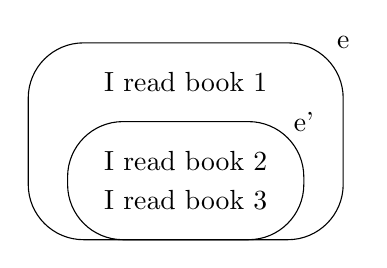
\begin{tikzpicture}
\draw [rounded corners = 20pt] (-2.5,0.5) rectangle (1.5,-2);
\draw [rounded corners = 20pt] (-2,-0.5) rectangle (1,-2);
\node at (1.5,0.5) {e};
\node at (1,-0.5) {e'};
\node at (-0.5,0) {I read book 1};
\node at (-0.5,-1) {I read book 2};
\node at (-0.5,-1.5) {I read book 3};
\end{tikzpicture}
\xe
%
Schein seems to consider the \quo{van Benthem} reading to be available. He wants a way to force readers to interpret the sentence within the big event $e$. He considers three ways to achieve this:

\pex
\a I read exactly two books in exactly 24 hours. \hfill (adverbial modifier)
\a I read exactly two books with the same title. \hfill (enriching descriptive content)
\xe
%
If $e'$ takes less than 24 hours and $e$ exactly 24 hours, then \clastx{a} can't possibly be talking about $e'$.

But Schein decides against these two ways of doing things

\begin{itemize}
\item Temporal adverbials because \quo{[they], one is prepared to concede, involve [quantification over] events in some crucial way}
\item \emph{same} because \quo{[they] hold mysteries of their own}
\end{itemize}
%
He prefers the following route which does the same thing that \emph{same} does with only material \quo{within the fragment that we are holding polyadic logical form responsible to}.

\section{Composition: quantifiers \& scope}

The truth conditions for \cref{quat} that we aim for should be true in the following scenario:

\ex \label{scenario}
\begin{center}
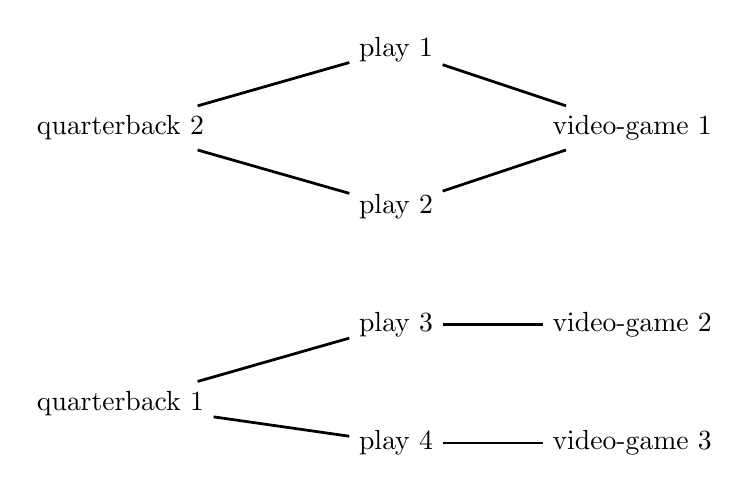
\begin{tikzpicture}
\node (v1) at (2.5,1.5) {video-game 1};
\node (v2) at (-0.5,2.5) {play 1};
\node (v4) at (-0.5,0.5) {play 2};
\node (v5) at (2.5,-1) {video-game 2};
\node (v6) at (-0.5,-1) {play 3};
\node (v7) at (2.5,-2.5) {video-game 3};
\node (v8) at (-0.5,-2.5) {play 4};
\node (v9) at (-4,-2) {quarterback 1};
\node (v3) at (-4,1.5) {quarterback 2};
\draw [line width = 1pt] (v1) edge (v2);
\draw [line width = 1pt] (v2) edge (v3);
\draw [line width = 1pt] (v1) edge (v4);
\draw [line width = 1pt] (v4) edge (v3);
\draw [line width = 1pt] (v5) edge (v6);
\draw [line width = 1pt] (v7) edge (v8);
\draw [line width = 1pt] (v8) edge (v9);
\draw [line width = 1pt] (v6) edge (v9);
\end{tikzpicture}
\end{center}
\xe
%


First off, the truth-conditions seem to imply that \emph{exactly two new plays} is in the scope of \emph{every}, since there are indeed two new plays per quarter back. That establishes on scope relation at least for our quantifier:

\begin{center}
every quarterback $\gg$ two new plays
\end{center}
%
Since there are two new plays \emph{per} quarterbacks, this imply, within Schein's view, that \emph{every} quantifies over singularities. The truth-conditions that the composition must give us will look as follows (unknowns in red, upper case variables range over pluralities, exactly 2 is left unanalysed):

\ex
$\text{\color{red} (three video games?)} \ldots \forall y\in \dbb{quarterback}, \text{Exactly 2 } Z\in \dbb{plays},  \dbb{give}({\color{red} ?})(y)({\color{red} ?})(e)$
\xe
%
Initially, Schein asks us to disregard the scope of the event closure (essentially closing it very locally). That being out of the way,
the real puzzle is \emph{three video-games}. Is it interpreted distributively, as a plural, or as something else? Relatedly, Schein leaves open the option of interpreting the two new plays distributively or not.

\paragraph{Option I: plural interpretation} The simplest option is to interpreted \emph{three video games} and \emph{exactly two new plays} as plural. This gives the following LF:

\ex\label{lf1}
$\exists X\in \dbb{video-games}, |X| = 3 \wedge \forall y\in \dbb{quarterback}, \underline{\text{Exactly 2 } Z\in \dbb{plays},  \dbb{give}(X)(y)(Z)(e)}$
\xe
%
Breaking down the evaluation of \clastx in manageable pieces, we first need to know of which $X$ and $y$ the underlined part is true. In other words, for each quarterback, we need to know which video-games taught him exactly two new plays. Schein provides the following answer:

\pex
\a for \emph{quarterback 1}, \emph{video-game 1} taught him exactly two plays
\a for \emph{quarterback 2}, \emph{video-game 2}$\oplus$\emph{video-game 3} taught him exactly two plays
\xe
%
One wonders why this is so. Couldn't we say that all three video-games taught \emph{quarterback 2} exactly two new plays? Sure, video-game 1 didn't contribute much to that but, as a group, they sure taught that quarterback two new plays.

Schein brushes off this team credit concern by pointing out that video-games are inanimate and need not have any particular link to each other to be true\footnote{Using the word \emph{team credit} kind of imposes restrictions on what we think the phenomenon is. Within that mindset, Schein's reply is valid. But if team credit is nothing but a special case of a more general mechanism of non-maximality, then it fails to adress the bigger question: could we get the three video-games to teach teach \emph{qurterback 2} exactly two new plays if we allow for non-maximality?}. If we accept his rebuttal, then \cref{lf1} indeed comes out as false, contrary to fact: there is no plurality $X$ that is related to every quarterback $y$ by two new plays.

In a nutshell, this LF requires the same set of video-games to have taught every quarterback. Schein brushes off other possible interpretations and notes that the correct truth-conditions can be paraphrased as follows:

\ex%
[each quarterback was \underline{taught} two new plays] and [the \underline{teachers} were three video-games]
\xe
%
This paraphrase can only be obtained if we have at least two operators in our LF, each encoding one of the two red predicates. This means some form of separation.


\paragraph{Option II: branching quantifiers}
\end{document}
